\documentclass[twocolumn]{article}
\usepackage{verbatim}
\usepackage{graphicx}
\usepackage{tabularx}
\usepackage{url}
\usepackage[htt]{hyphenat}

\newcommand{\naive}{Na\"\i ve}
\newcommand{\method}[1]{\texttt{#1()}}
\newcommand{\class}[1]{\texttt{#1}}
\newcommand{\param}[1]{\texttt{#1}}
\newcommand{\aicat}{\texttt{AI::Cat\-e\-gor\-i\-zer}}


\title{Streamlined Automatic Categorization of Mathematics Questions}

\author{
{\em Ken Williams}\\[1ex]
Web Engineering Group\\
The University of Sydney\\
Bldg J03, Sydney NSW 2006\\[1ex]
{\em kenw@ee.usyd.edu.au}
\and
{\em Rafael A. Calvo}\\[1ex]
Web Engineering Group\\
The University of Sydney\\
Bldg J03, Sydney NSW 2006\\[1ex]
{\em rafa@ee.usyd.edu.au}
\and
{\em David Bell}\\[1ex]
Web Engineering Group\\
The University of Sydney\\
Bldg J03, Sydney NSW 2006\\[1ex]
{\em dave@student.usyd.edu.au}
}

\begin{document}

\maketitle
\thispagestyle{empty}


\subsection*{\centering Abstract}
\noindent
{\it 
This paper describes a new approach to managing a stream of questions about 
mathematics by integrating a text categorization framework into a relational database 
management system. The corpus studied is based on unstructured submissions to an 
ask-an-expert service in learning mathematics. The classification system has 
been tested using a \naive\ Bayes learner built into the framework. The 
performance results of the classifier are also discussed. The framework was integrated 
into a PostgreSQL database through the use of procedural trigger functions.
}

\paragraph{Keywords} 
Tutoring Systems, Learning Communities, Document Management, Automatic
Text Categorization



\section{Introduction}

Ask-an-expert services are becoming more common, spanning from standard 
customer relationship management to discussion forums in a particular discipline. In 
general, these online services are supported by domain experts who attempt to answer 
questions posted via email or web forms. Since these experts often have a single subdomain of expertise it is 
very helpful if they have only to read questions that relate to this subdomain. This can be 
done by organizing the service in such a way that users are encouraged to post their 
question in the appropriate area. However, this approach is not always successful as 
often the user will either ignore the organization scheme or not know to which area their 
question belongs. 

These problems are common within a number of domains. Our test was performed on 
messages sent to a mathematics ask-an-expert
service for students and teachers.\cite{drmath} The issues 
discussed also apply to other similar systems such as customer relationship 
management (CRM) and e-learning systems in general. These systems can use an 
automatic text categorization framework to categorize the questions into the experts' 
area of interest, or into the appropriate customer support mailbox. 

The downside of an automatic categorization approach is that integrating such 
functionality into existing systems can be very complex, and often involves an in 
depth understanding of text categorization techniques.  Also, the content is normally 
stored in systems with a relational database in the backend, as is the case for most 
content and learning management systems. By building the categorizer into the 
database, the categorization framework\cite{williams:02} can be made invisible to the 
users and is thus more attractive to the average system administrator or application 
developer. Also, application developers, do not have to re-implement the 
classification software. They only need a machine learning professional to assist in 
training the classifier, and once trained it can then be reused in different applications. 

The applications of information retrieval have been well studied since the 1980s, as 
discussed by Salton \cite{salton:89,salton:91}, and many of these methodologies have been 
integrated into commercial database management systems that have free text search 
capabilities. However, this integration does not seem to have penetrated the text 
categorization domain.

Section 2 of the paper discusses the data set that was used to test
the system. Section 3 discusses the text categorization framework and
the extensions made to it, including the implementation within the
database management system. Section 4 discusses the quantitative
results of the testing process and Section 5 concludes.

\section{Dr. Math Corpus}
\label{corpus}

For the evaluation of our system we have tested the performance of the
categorization system over a set of unstructured, informal documents
from the Ask Dr. Math service.\cite{drmath} These documents are mostly
written by students between the ages of 6 and 18, though question
submissions can come from any member of the general public.  The documents vary
in length from a single sentence to several paragraphs. In addition to
this, many examples contain symbols and diagrams, making linguistic
analysis very difficult. The Ask Dr. Math service has about 300
volunteers (about 30-40 of which may be active in any given month),
dealing with hundreds of questions a day. The volunteers have
expertise in different areas of math, and the site has won a number of
awards for its useful service.

The filtering of questions is a major element of the Ask Dr. Math
question answering process.  The service may receive about 7000
questions a month, about half of which are eventually answered.  The
unanswered questions may be duplicate submissions, messages of thanks,
inappropriate questions, or other messages that don't require a
response.  There also may be some legitimate mathematics questions
that go unanswered, simply because the service is not fee-based for
either the students or the experts, and thus can make no guarantee
that any particular question will be answered.  The experts are
currently responsible for choosing their own questions to answer.

The Dr. Math corpus we used contains 6632 documents and was split into a training
set of 5305 documents and a testing set of 1327 documents.  There are 95 categories 
in the corpus. The average number of documents in each category is
107.15.  The most popular category, high school-level geometry,
contains 877 documents, and the least popular category,
elementary-level golden ratio, contains only 3 documents.  Each
document may be a member of more than one category, and the average
number of categories per document is 1.53.  Figure
\ref{cat-distribution} shows the distribution of categories throughout
the corpus.  Category names indicate both level and topic, such as
``geometry.elem'' or ``calculus.college.''

\begin{figure}
\begin{verbatim}
Implicit Differentiation

Find the slope of the tangent at the point
(3,4) on the circle x^2 + y^2 = 25.

My answer: I guess we would need to put it
in the y = mx + b form. 

Thanks for any help,
Scott
\end{verbatim}
\caption{An example document from the Dr. Math corpus}
\end{figure}

It may be important to note that our corpus was drawn from the public
archive of answered questions, not directly from the stream of
incoming questions.  Because the archiving process is fairly intensive
and not all questions are chosen for archiving, our corpus may
therefore differ significantly from the incoming question stream.  For
example, none of the kinds of unanswered questions mentioned earlier
are represented in the archive.  Because of this difference, it is
difficult to extrapolate our experiments to performance on the
incoming question stream.  However, because the incoming question
stream is uncategorized, obtaining a large enough number of
categorized questions for our investigation necessitated drawing them
from the archived questions.

\begin{figure}
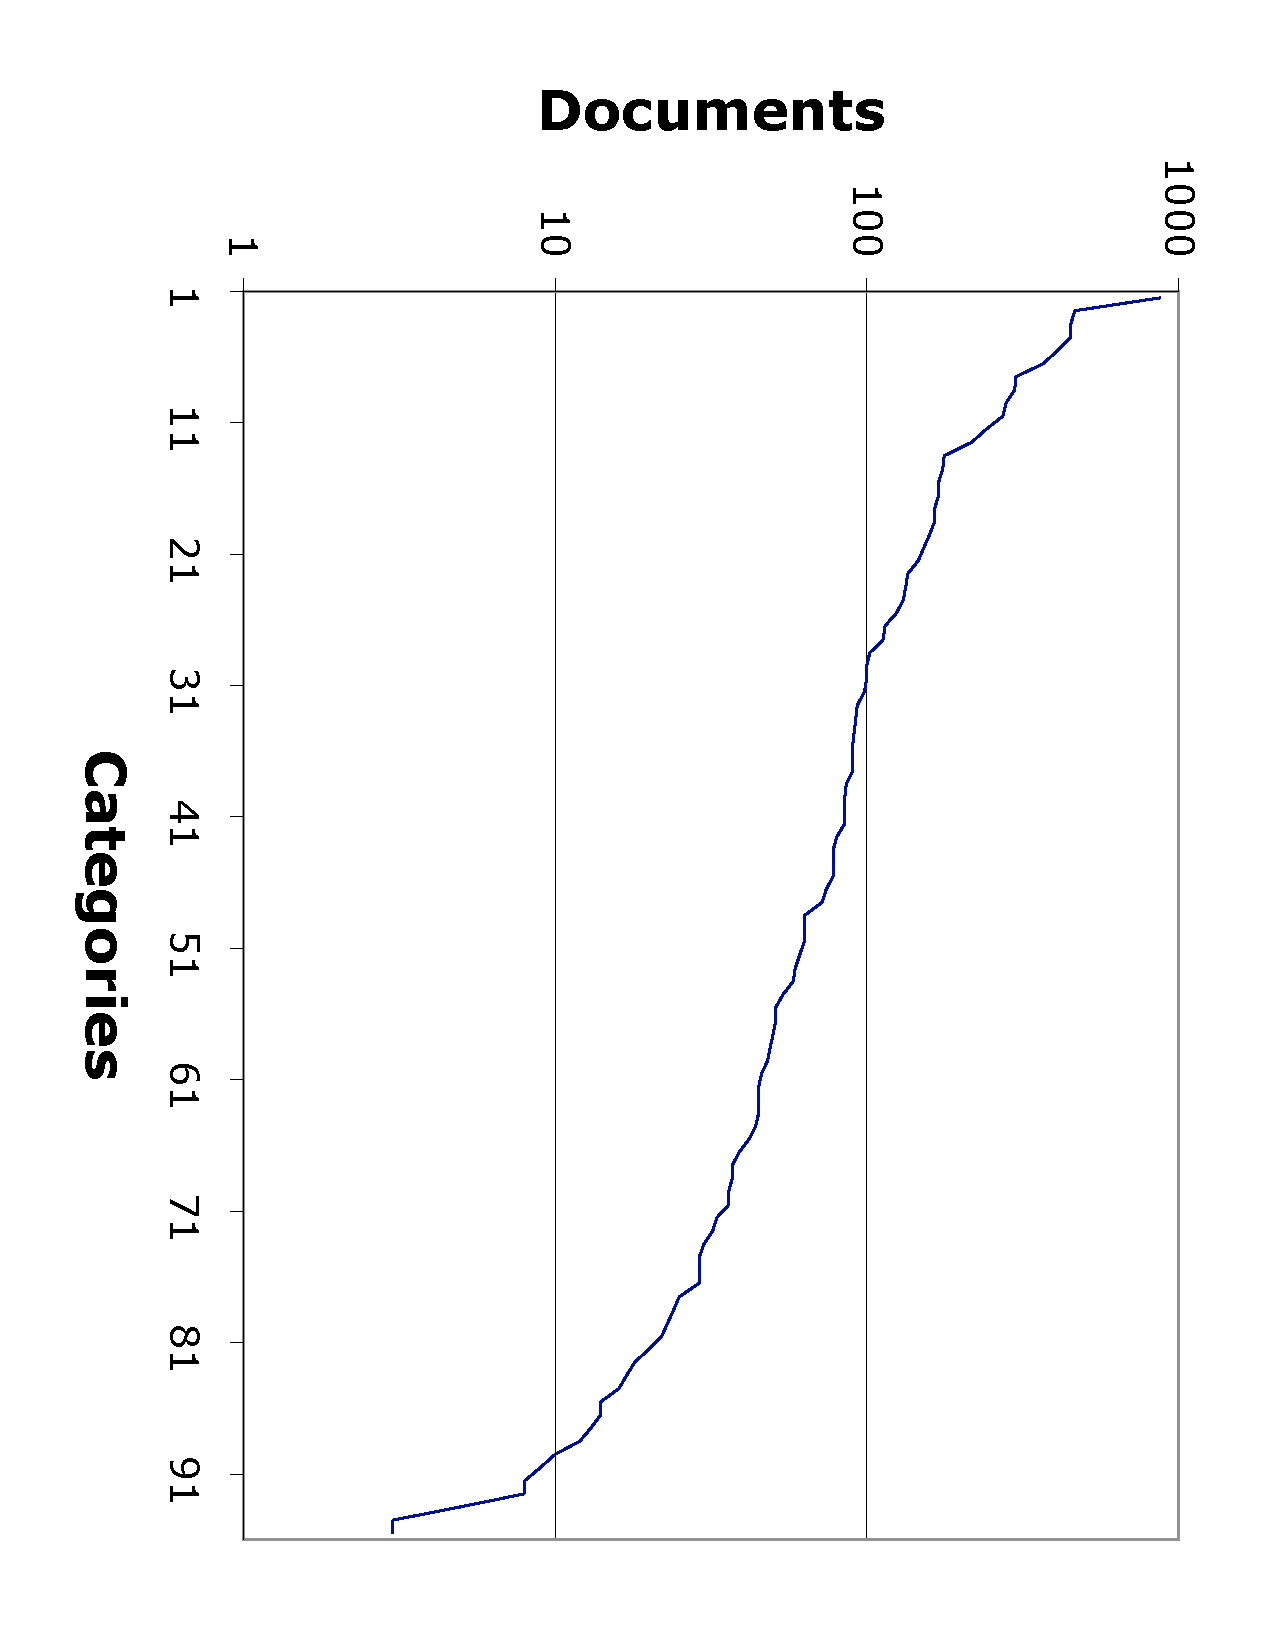
\includegraphics[angle=90,width=\linewidth]{cat-distribution}
\caption{Category distribution for the 95 Dr. Math categories}
\label{cat-distribution}
\end{figure}


\section{Categorization Framework}

Object Oriented Application Frameworks (OOAF) are software engineering artifacts 
that improve reusability of design and implementation \cite{fayad:97, fayad:99}.

The framework used in this project was designed to provide a
consistent way to build document categorization
systems.\cite{williams:02} It allows the developer to focus on the
quality of the more critical and complex modules by allowing reuse of
common, simple base modules.  The framework already has
implementations of Support Vector Machine (SVM), \naive\ Bayes, and
Decision Tree classifiers \cite{yang:99, sebastiani:02}. Other methods
such as Neural Networks \cite{calvo:00, calvo:01} and
K-Nearest-Neighbor classifiers are under development.

In this project we extended the framework by adding an alternative
Collection class to allow for the data to be read directly from a
database instead of from a file system.  Framework extensions are built by subclassing
the main classes in the framework. Class inheritance contributes to code reuse and 
quality. The framework also provides statistical analysis of experimental results, and 
produced the performance measures discussed in Section \ref{results}.

The framework's architecture and language choice enabled us to easily build the 
framework into postgreSQL through postgreSQL's PL/Perl and PL/perlU support. 
This support allows the creation of procedural language functions through the use of 
the "CREATE FUNCTION" SQL command. Using this support and the PL/perlU language 
we were able to build a "launching" function that invoked the categorization 
framework on the document to be classified. This means that the only command 
necessary to categorize a document is a basic insert statement with a function call in 
place of a value for the category of the document, as shown in Figure \ref{sql-insert}.
This statement can be further simplified through the creation of a pl/psql 
trigger function which fires automatically on insertion and passes the necessary values 
to the \method{categorize} function.

\begin{figure}
\begin{verbatim}
 INSERT INTO documents
  (name, content, categories) 
 VALUES
  ('my name',
   'my content',
   categorize('my name',
              'my content',
              'documents'));
\end{verbatim}
\caption{Example document insertion statement with categorization}
\label{sql-insert}
\end{figure}

If the categorization is to take place within a database, where
categorized documents are often going to be appended to the learning
set, a learning algorithm which has very little training overhead is
ideal.  This avoids the need to retrain a categorizer after each
document insertion.  Two such algorithms are the \naive\ Bayes
algorithm (NB) and the K-Nearest Neighbor algorithm (kNN).

The training phase in NB consists only of counting term frequencies in
each document and using them to calculate conditional probabilities
between terms and categories.  These probabilities are then consulted
when categorizing a new document, with conditional probabilities for
each term being multiplied to find the probability that a given
document belongs to a certain category.

kNN in its basic form has essentially no training phase.  Each
document is represented as an $n$-dimensional vector, where $n$ is the
number of unique terms in the training set.  When a new document is to
be classified, it is compared to the vectors of the documents in the
training set. The $k$ training vectors which are closest to the test
vector are found (with distance defined as the cosine of the angle
between any two vectors), and the most prevalent category or
categories amongst these is assigned to the new document.

In our testing, we have found that NB is a more accurate categorizer
than kNN.  This seems contrary to the findings of \cite{yang:99}, and
may reflect the fact that our implementation of NB is more mature than
our kNN implementation.  The rest of this paper will focus on the NB
experiment and results.

Since the categorization performance is determined only by the classification 
framework, all these methods should behave the same inside the
database as they do outside 
the database. What the integration into the database does is to make the 
functionalities of the framework available as procedures in the SQL language.
Since relational databases can be designed using an object oriented methodology \cite{blaha:88,
rumbaugh:91}, by integrating it in this way, the classification task 
(and framework) can also be designed into larger OO systems.

\section{Method and Results}
\label{results}

The 5305 training documents in the Dr. Math corpus were loaded into a database 
table named ``documents.'' This table consisted of 3 columns: name, content and 
categories. The testing set was then inserted into the database, one document at a time 
using a statement similar to that in Figure \ref{sql-insert}. After each insert a SELECT query was 
run to extract the assigned categories. These categories were then compared to the 
actual categories of that document. Through this comparison the performance of the 
categorization in terms of recall  and performance  was measured. The precision and 
recall\footnote{Recall is the proportion of the target items that the
system selected, i.e. tp/(tp+fn).  Precision is the proportion of
selected items the system got right, i.e. tp/(tp+fp).} were then used
to calculate the $F_1$ measure \cite{calvo:01,sebastiani:02}.

\begin{table}
\begin{tabular}{|r|r|r|r|r|r|}
\hline
         & $MaP$   & $MaR$   & $MaF_1$ & $MiF_1$ & Error \\ \hline
NB       & 0.246   & 0.226   & 0.226   & 0.361   & 0.022 \\ \hline
kNN      & 0.211   & 0.186   & 0.179   & 0.257   & 0.025 \\ \hline
Baseline & 0.019   & 0.018   & 0.018   & 0.042   & 0.031 \\ \hline
\end{tabular}
\caption{Macro- and Micro-averaged performance scores.}
\label{results-main}
\end{table}


The results in Table \ref{results-main} show the performance of the
categorization algorithms.  The precision, recall, and $F_1$ scores
can be computed using macro-averaging, which gives equal weight to
each category, or micro-averaging, which gives equal weight to each
document. \cite{yang:99, sebastiani:02} For the kNN algorithm, we used
a $k$ value of 15 and a categorization threshold of 0.12, which seemed
to perform the best in our investigations.  We also include in Table
\ref{results-main} the results of a baseline classifier, which simply
assigns categories randomly to each test document based on the
frequency of categories in the training set.

Next, we turned our attention to ways of improving performance on the
test set.  As mentioned in Section \ref{corpus}, each category name is
a combination of two components, a level and a topic.  This suggests
that separate categorizers could be trained to recognize the two
components separately, perhaps with more success than a single
categorizer may have on the two components together.

Table \ref{results-NB} shows the success of a \naive\ Bayes
categorizer, and Table \ref{results-baseline} shows a baseline
categorizer for comparison.  We give results for the level task, the
topic task, and a task that uses the separate topic and level
categorizers to assign a combined category.

Comparing the combined task to the NB results in Table
\ref{results-main}, we see that separating the categorization task
into two subtasks hurt overall performance on the combined task.  The
level task looks promising, but comparing it with the baseline
categorizer shows that it may not be significantly better than random
guessing.  However, the performance on the topic task is noteworthy,
because it is so far above both the baseline categorizer and the
original NB categorizer.  In addition, the topic assignment may be
more valuable than the level assignment, because while most students
will be able to indicate their own age or grade level when asking a
question, they may not be able to place their own question in an
appropriate category.

Because the math topics used in this experiment were generated from
the category names, we ended up with some duplication that may have
hurt performance.  For example, there are categories called
``probability.high,'' ``statistics.high,'' and ``prob.stats.middle.''
This means that the combined list of extracted math topics includes
``probability,'' ``statistics,'' and ``prob.stats.''  The exact effect
of this on the categorizers is unknown, but we might expect these
overlapping categories to confuse the categorizer.  A service such as
this one may therefore benefit from using more consistent category
names.


\begin{table}
\begin{tabular}{|r|r|r|r|r|r|}
\hline
Task     & $MaP$   & $MaR$   & $MaF_1$ & $MiF_1$ & Error \\ \hline
Level    & 0.524   & 0.626   & 0.570   & 0.671   & 0.223 \\ \hline
Topic    & 0.339   & 0.314   & 0.313   & 0.440   & 0.026 \\ \hline
Both     & 0.187   & 0.181   & 0.166   & 0.223   & 0.035 \\ \hline
\end{tabular}
\caption{Performance of \naive\ Bayes classifier on subtasks.}
\label{results-NB}
\end{table}

\begin{table}
\begin{tabular}{|r|r|r|r|r|r|}
\hline
Task     & $MaP$   & $MaR$   & $MaF_1$ & $MiF_1$ & Error \\ \hline
Level    & 0.326   & 0.319   & 0.322   & 0.468   & 0.328 \\ \hline
Topic    & 0.029   & 0.027   & 0.027   & 0.067   & 0.041 \\ \hline
Both     & 0.015   & 0.010   & 0.011   & 0.035   & 0.027 \\ \hline
\end{tabular}
\caption{Performance of baseline classifier on subtasks.}
\label{results-baseline}
\end{table}


 
\section{Conclusion}

We have described a system that integrates a categorization framework into a 
relational database. The results show it is possible to integrate categorization 
techniques into the relational databases used by learning and content management 
systems.

Two categorization algorithms were applied to the task of classifying
messages sent to an educational ask-an-expert service.  A \naive\
Bayes classifier was fairly successful at categorizing the messages.
The highest success rate was found in classifying messages by math
topic, a task that coule be useful on the unstructured data sent to
services such as the one we discussed.

\section*{Acknowledgements}

The authors gratefully acknowledge financial support from the Capital Markets 
Collaborative Research Centre and the University of Sydney. The authors also 
acknowledge The Math Forum for giving permission to use and discuss their data. 

\bibliographystyle{plain}
\bibliography{TC-references}

\end{document}
